\section{Funktionelle krav}\label{funktionellekrav}
\textit{...}

Formålet med systemet er, at udvikle en aktivitetsmåler som har potentialet til at reducere antallet af inaktive børn i aldersgruppen 9-12 år. Dette gøres med henblik på at ændre den teknologiske udviklings påvirkning af børns aktivitetsvaner fra inaktivitet til aktivitet.
Der ønskes derfor et analogt system som detekterer aktiviteterne gang, løb og cykling, da disse er gængse aktiviteter i et barns hverdag. Måden hvorpå et analogt system kan detektere disse aktiviteter kan ske gennem accelerometre og gyroskoper, hvorefter systemet, gennem algoritmer, skal kunne adskille gang, løb og cykling.
Hertil skal intensiteten af aktiviteterne registreres igennem puls, da dette giver en indikation af det fysiologiske udbytte, barnet får ud af en given aktivitet. Herved vil det blandt andet kunne registreres om barnet er aktiv med høj intensitet i de anbefalede 30 minutter tre gang om ugen, som beskrevet i \secref{subsec:fysio_aktivitet}. \newline
For at systemet har en motiverende effekt på børn, skal der være en brugerflade som børnene finder interessant. Denne skal give feedback på dagens samlede præstationer samt progressionen i aktivitetsniveauet.

Systemet skal kunne detektere børns aktivitet igennem en hel dag, uden at være til gene, hvorfor det skal kunne fungere uafhængigt af andre systemer. Det skal derfor være et trådløst system, som kan sende data til en ekstern enhed og er batteridrevet med en dags levetid. Derudover skal det være elektrisk sikkert, således at barnet ikke kan komme til skade som følge af aktivitetsmålerens design. 

Brugeren får feedback på sin præstation gennem en visualisering af dataet fra aktivitetsmåleren, hvorfor dataet behandles i den eksterne enhed. \newline
Før dataet kan blive behandlet og sendt til den eksterne enhed, skal det konverteres fra analoge signaler til digitale signer. 

På baggrund af ovenstående, udformes de funktionelle krav til systemet, således: 
\begin{itemize}
	\item Systemet skal gennem sensorer kunne detektere aktiviteterne gang, løb og cykling.
	\item Systemet skal gennem algoritmer i softwaren kunne adskille gang, løb og cykling.
	\item Systemet skal kunne registrere intensiteten af de givne aktiviteter igennem puls.
	\item Systemet skal være komfortabelt, hvorfor det trådløst skal kunne videresende signaler til en ekstern enhed og være batteridrevet over en hel dag.
	\item Systemet skal være elektrisk sikkert for brugeren.
	\item Signalerne som er sendt til en ekstern enhed, skal behandles og repræsenteres visuelt.
	\item Systemet skal motivere børn i aldersgruppen 9-12 år. 
\end{itemize}

\subsection{Blokdiagram}
Ud fra de funktionelle krav til systemet, udformes et blokdiagram. \newline
Af blokdiagrammet på \figref{fig:blokdiagram}, fremgår rækkefølgen af blokkene samt om de er analoge eller digitale dele. 

Den analoge del, som er omringet af en rød firkant på \figref{fig:blokdiagram}, består af inputs fra de tre analoge sensorer; accelerometer, gyroskop og pulssensor. Disse analoge inputs konverteres fra analoge til digitale signaler gennem en ADC. Herefter skal en algoritme herefter adskille de digitale signaler for de tre aktivitetsformer fra hinanden, hvilket sker i den digitale del ved sensorerne, som er omringet af en grøn firkant på \figref{fig:blokdiagram}. Det digitaliserede data fra de tre sensorer sendes trådløst til en ekstern enhed, hvor det behandles og repræsenteres visuelt. 

 \begin{figure}[H]
 	\centering
 	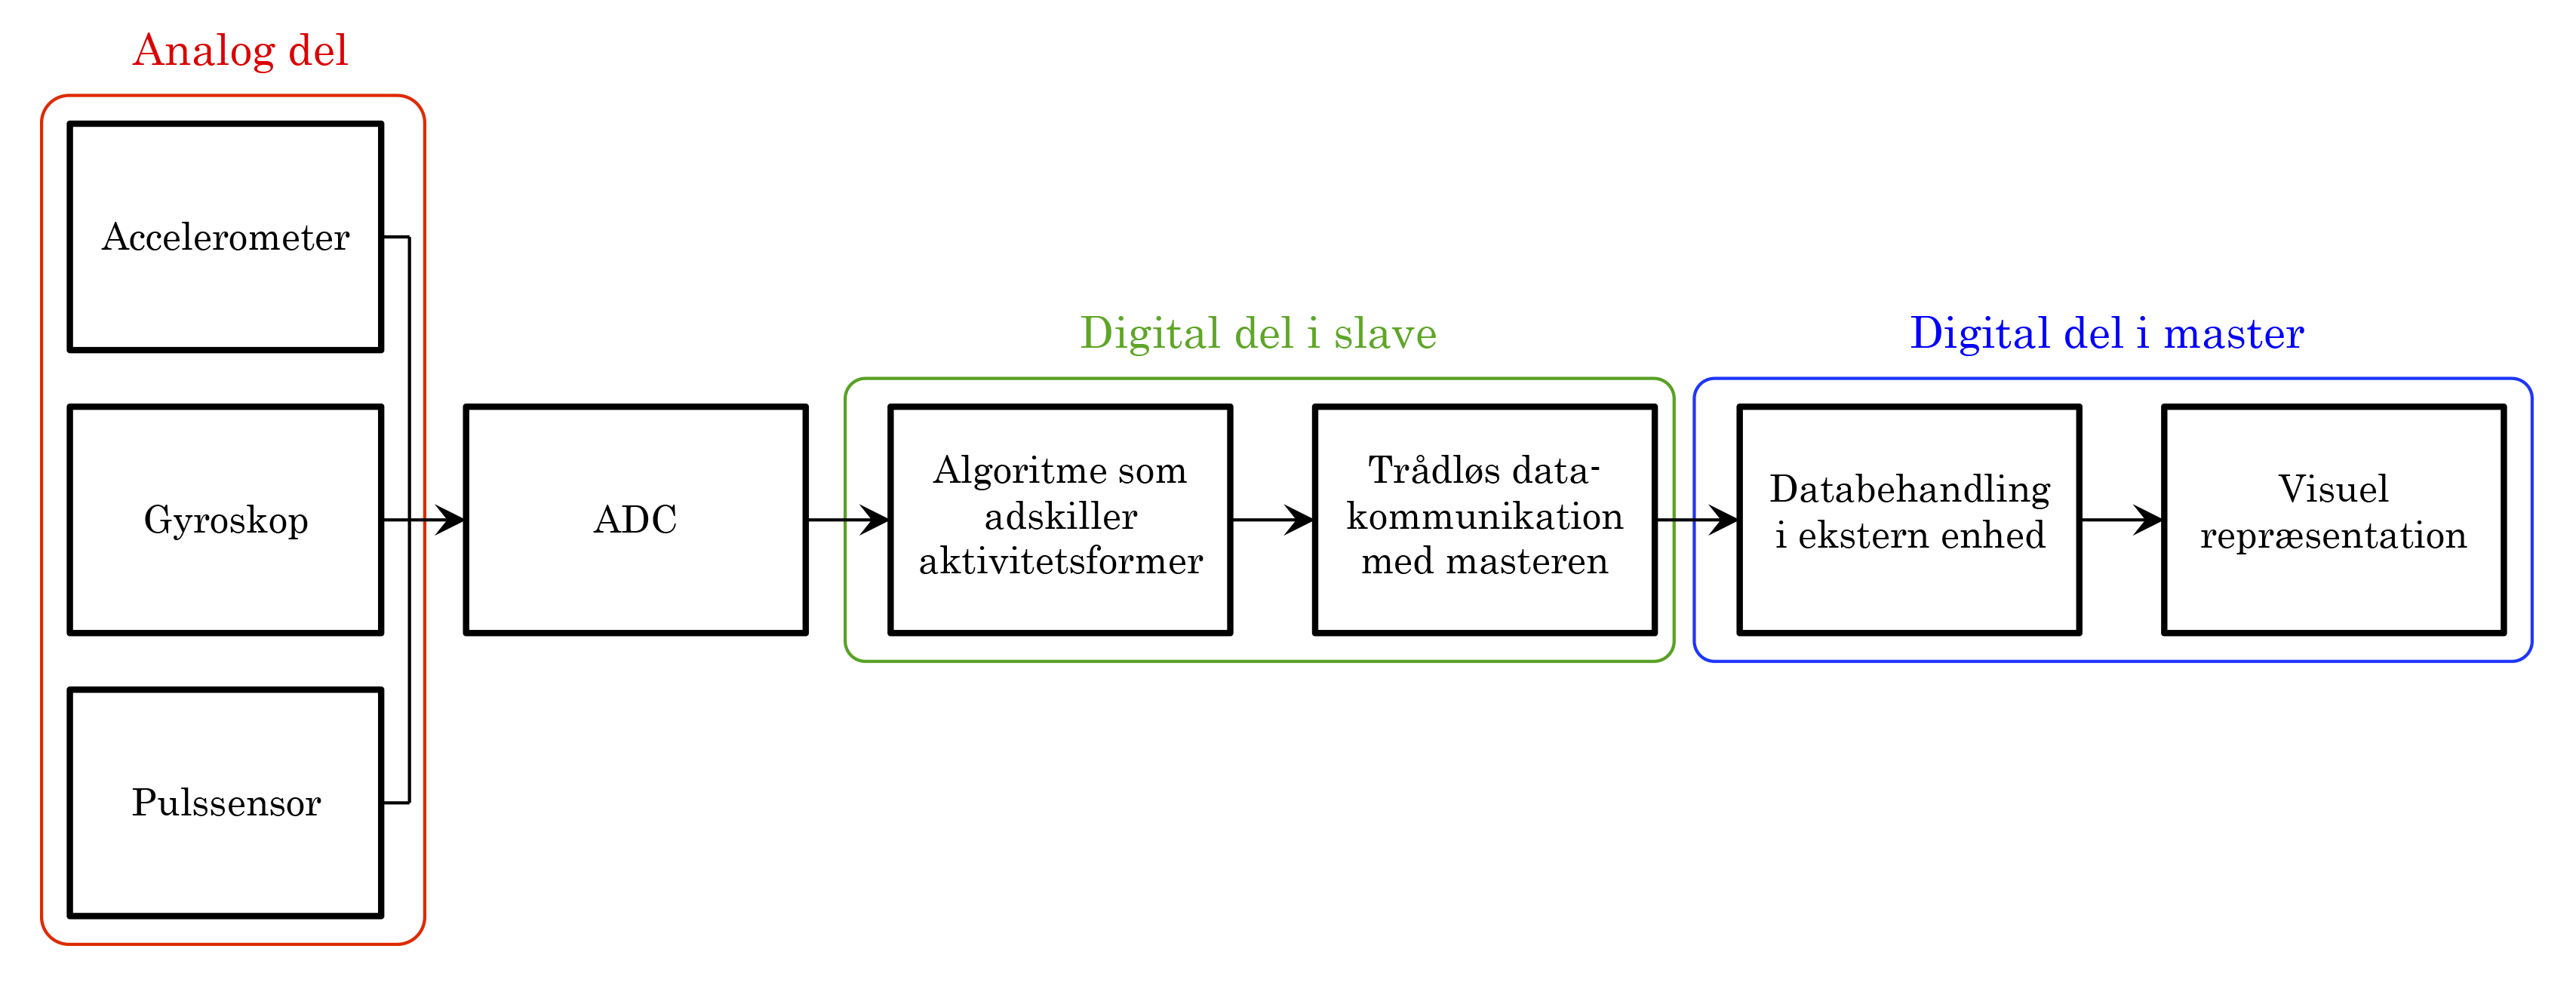
\includegraphics[scale=0.54]{figures/bProblemloesning/blokdiagram2.png}
 	\caption{Blokdiagram for systemet}
 	\label{fig:blokdiagram}
 \end{figure}
 \fxnote{Burde det være en pil beggeveje til gyroskop og accelerometer?}